\subsection{Used Tools and Frameworks}
\label{subsec:used_tools_frameworks}

For the development of the Communication Hub, our team utilized the Robot Operating System (ROS) 1 as the primary framework. ROS is an open-source software framework that provides a high-level abstraction of the robot's functionality, allowing developers to focus on the implementation of the robot's behavior rather than the underlying hardware.


\subsubsection{Advantages of ROS}

The primary intention behind developing the ROS framework was to create a generic software framework for robots, enabling collaboration and reusability across different robotic systems. In contrast to earlier robotics research, where software was often exclusive to specific robots, ROS offers a flexible and modular platform.

ROS excels in several aspects, including:

\subsubsection{Collaborative Development}

As an open-source and free framework, ROS fosters collaborative development among industries and research institutions. Its modular design allows developers to expand its functionalities by adding packages, which can be easily reused for other robots due to the hardware abstraction layer.

\subsubsection{Language Support}

The ROS communication framework can be easily implemented in various modern languages, including C++, Python, Lisp, and others, providing developers with the flexibility to work with their preferred language.

\subsubsection{Library Integration}

ROS provides an interface to numerous third-party robotics libraries, such as Open-CV, PCL, Open-NI, Open-Rave, and Orocos, enabling seamless integration and utilization of these libraries.

\subsubsection{Simulator Integration}

ROS has ties to open-source simulators like Gazebo and interfaces with proprietary simulators like Webots and V-REP, allowing developers to test and simulate their applications in a realistic and controlled environment.

\subsubsection{Code Testing}

ROS offers an inbuilt testing framework called rostest, which enables developers to check code quality and detect bugs, ensuring robust and reliable application development.

\subsubsection{Scalability}

The ROS framework is designed to be scalable, allowing developers to perform heavy computation tasks on robots using cloud-based or heterogeneous cluster-based architectures, making it suitable for complex and demanding applications.

\subsubsection{Customizability}

As an open-source and free framework, ROS can be customized to meet specific robot requirements. Developers can remove or modify components to suit their needs, ensuring optimal performance and adaptability.

\subsubsection{Community}

ROS is a community-driven project led by OSRF, with a large and active community supporting its development. This community provides a valuable resource for developers, offering guidance and support throughout the application development process \cite{joseph2017ros}.


ROS provides functionality for hardware abstraction, device drivers, communication between processes over multiple machines, tools for testing and visualization, and much more. The key feature of ROS is the way the software is run and the way it communicates, allowing you to design complex software without knowing how certain hardware works.
\subsubsection{ROS 1 Core (Master)}
\begin{figure}[h]
\centering
\includegraphics[width=0.8\textwidth]{Figures//CentralProcessingNode//UsedToolsAndFrameworks//Ros_images/ros_1_architecture_diagram.png}
\caption{ROS 1 Architecture Diagram}
\end{figure}

The ROS 1 core, also known as the ROS master, is the central component of the ROS system. It is responsible for managing the ROS graph, which is a collection of nodes, topics, and services that make up the ROS system. The ROS master provides a registry of available nodes, topics, and services, and enables nodes to discover and communicate with each other \cite{fairchild2016ros}.

The ROS master is responsible for:

\begin{itemize}
\item Node registration: nodes register with the ROS master to announce their presence and capabilities.
\item Topic registration: topics are registered with the ROS master to enable nodes to publish and subscribe to them.
\item Service registration: services are registered with the ROS master to enable nodes to provide and use them.
\item Node discovery: nodes can discover other nodes and their capabilities through the ROS master.
\end{itemize}

For a simple example of the ROS Master in action, see the ROS wiki page at \url{http://wiki.ros.org/Master}.

In our project, we utilized the ROS 1 core to manage the Communication Hub's nodes and topics. The ROS master enabled us to easily add or remove nodes, and to manage the communication between them.

\subsubsection{ROS Nodes}

In ROS, nodes are the basic execution units that perform specific tasks. They can be thought of as individual programs that communicate with each other using ROS messages. Nodes can be grouped into packages, which can then be easily shared and distributed among ROS users \cite{fairchild2016ros}.


In our project, we utilized multiple nodes to achieve the Communication Hub's objectives. Each node was responsible for a specific function, such as sensor data processing, actuator control, or data visualization. By using nodes, we were able to separate concerns into their respective nodes, while still empowering the robot to make complex decisions to execute a task.

\subsubsection{Popular ROS Topics}

In ROS, communication between nodes on a specific topic uses the same message type for both publishers and subscribers, as illustrated in Figure 4-2. When a subscriber node registers for a topic with the Master, it receives information about the corresponding publisher node. The subscriber node then establishes a direct connection with the publisher node to receive messages.

For instance, in a mobile robot application, the current position of the robot can be calculated from encoder values and published as odometry information using a topic message (x, y, i). This asynchronous information can be continuously transmitted in a unidirectional flow, making it suitable for sensor data that requires periodic publishing.

One of the key benefits of topics is that they are unidirectional and remain connected, enabling continuous message transmission. Additionally, multiple subscribers can receive messages from a single publisher, and multiple publishers can send messages to a single subscriber. This flexibility allows for multiple connections between publishers and subscribers, making it a powerful communication mechanism in ROS\cite{pyo2017ros}.

\begin{figure}[h]
\centering
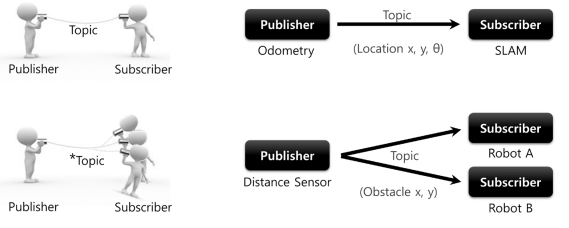
\includegraphics[width=0.8\textwidth]{Figures//CentralProcessingNode//UsedToolsAndFrameworks//Ros_images/RosTopic.png}
\caption{Example of a ROS Topic}
\end{figure}

By leveraging ROS 1 and its node-based architecture, we were able to create a robust and efficient communication system for our robot. The use of ROS enabled us to focus on the implementation of the robot's behavior, rather than the underlying hardware, and to easily integrate and test various components and algorithms.
%End_Of_Yossry_Part